
\chapter{Virtual Machine}

\section{Development Environment}

\paragraph{} The BigDuck compiler will be developed using the Go programming
language. Antlr4 will be used as lexer and parser generator. And it will be
developed on MacOS, any other system support is not considered. Nevertheless
with access to a Go compiler and ANTLR, it should be possible to run the
BigDuck compiler however this has not been tested.

\section{Memory Management}
\subsection{Architecture}

\paragraph{} The BigDuck virtual machine is influenced by the architecture used
by the MOS 6502 8-bit microprocesor (mainly because this was the one we study
in depth on the Computer Organization course). The features taken directly from
this processor are the usage of stack pointers to handle function calls
and recursion, and the usage of a program counter to keep track program
execution.

\paragraph{} There are three components, the \emph{virtual} machine which is
the one that manages program execution, the \emph{memory} which stores all
values and has stack pointers to handle contexts, and the \emph{memory stack}
which stores the frame sizes used by each context.

\newpage

\begin{figure}[h]
    \centering
    \caption{Architecture Diagram}
    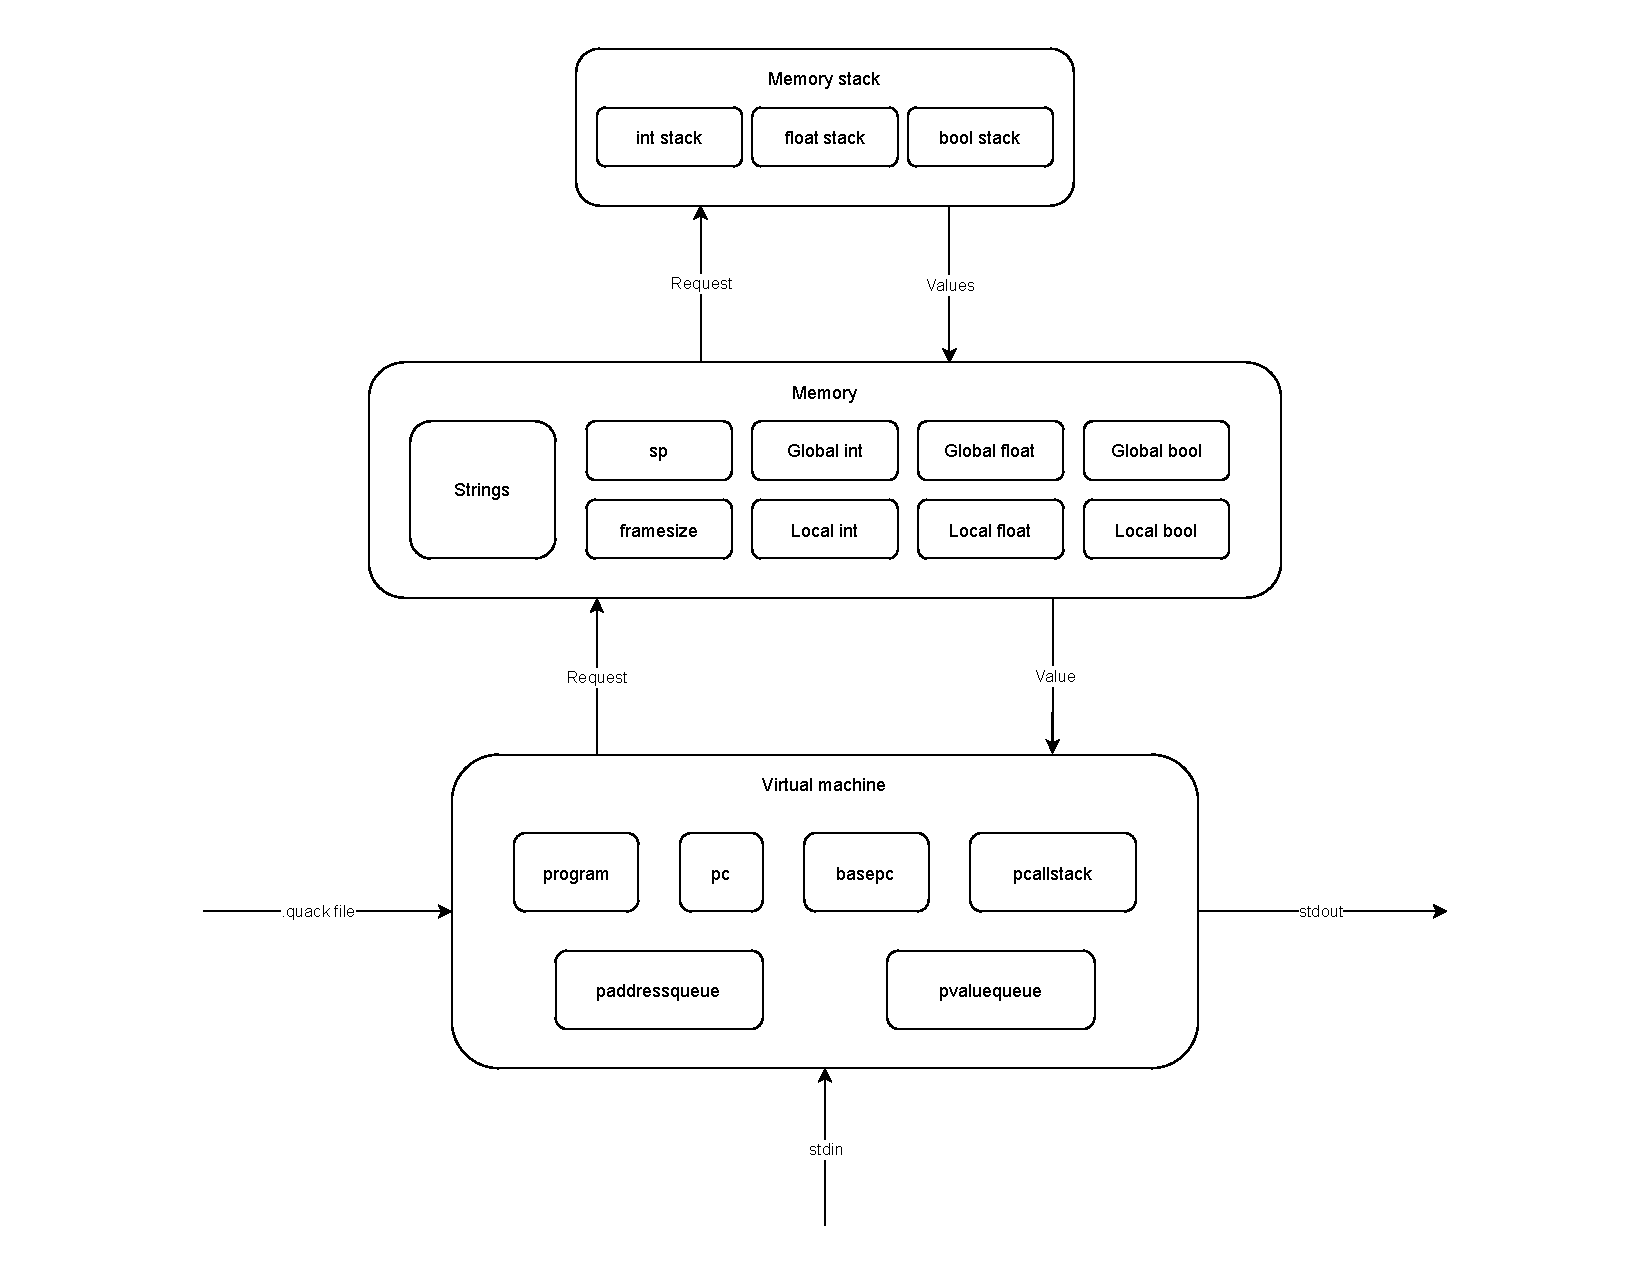
\includegraphics[trim={1.80in 0 1.80in 0},width=\textwidth]{vm_architecture}
\end{figure}

\newpage

\subsection{Data Structures}

\subsubsection{Virtual machine}

\begin{figure}[h]
    \centering
    \begin{tabular}{p{1in}p{3in}}
        \toprule
        \textbf{Element} & \textbf{Description}\\
        \midrule program &
        Array of three-address code structures which contains \newline program
        instructions.\\

        \midrule pc &
        Program counter, keeps track of the current instruction to execute.\\

        \midrule basepc &
        Base program counter, points to the beginning of the program segment on
        the executable.\\

        \midrule pcallstack &
        Procedure call stack, stores the next pc value before jumping to a
        procedure's code.\\

        \midrule paddressqueue &
        Parameter address queue, stores the addresses of the parameters given
        to a procedure.\\

        \midrule pvaluequeue &
        Parameter address queue, stores the value of the parameters given
        to a procedure.\\

        \bottomrule
    \end{tabular}
\end{figure}

\subsubsection{Memory}

\begin{figure}[h]
    \centering
    \begin{tabular}{p{1in}p{3in}}
        \toprule
        \textbf{Element} & \textbf{Description}\\
        \midrule strings &
        Stores string values.\\
        
        \midrule sp &
        Stack pointer, points to the beginning of the frame on each memory
        pool.\\
        
        \midrule framesize &
        Stores the size of the current frame.\\
        
        \midrule Local and global \newline pools &
        For each type, there are 2 pools to maintain the values used in each
        scope.\\
        
        \bottomrule
    \end{tabular}
\end{figure}

\subsubsection{Memory Stack}

\begin{figure}[h]
    \centering
    \begin{tabular}{p{1in}p{3in}}
        \toprule
        \textbf{Element} & \textbf{Description}\\
        \midrule Type stack &
        Stores the framesizes used by each procedure call.\\
        
        \bottomrule
    \end{tabular}
\end{figure}

\newpage

\subsection{Virtual Address Translation}

\paragraph{} The following enumerations were already used throughout
compilation.

\paragraph{Scope enumeration}

\begin{align*}
    \texttt{0} &\ \texttt{local}\\
    \texttt{1} &\ \texttt{global}\\
\end{align*}

\paragraph{Type enumeration}

\begin{align*}
    \texttt{2} &\ \texttt{0010}\ \texttt{int}\\
    \texttt{3} &\ \texttt{0011}\ \texttt{float}\\
    \texttt{4} &\ \texttt{0100}\ \texttt{bool}\\
    \texttt{5} &\ \texttt{0101}\ \texttt{string}\\
\end{align*}

\paragraph{} Therefore it seemed natural to used it as flags on a bit mask
in order to assign the virtual addresses.

\paragraph{Memory map}

\begin{align*}
    \texttt{1} &\ \texttt{scope bit}\\
    \texttt{3} &\ \texttt{type bits}\\
    \texttt{7} &\ \texttt{address nibbles}\\
\end{align*}

\paragraph{Examples}
\begin{align*}
    \texttt{0010}\ \dots\ \texttt{0000 0000}
    &\rightarrow \texttt{local int at address 0}\\
    \texttt{1011}\ \dots\ \texttt{0000 1010}
    &\rightarrow \texttt{global float at address 10}\\
    \texttt{0100}\ \dots\ \texttt{0001 0110}
    &\rightarrow \texttt{local bool at address 22}\\
    \texttt{1101}\ \dots\ \texttt{0000 1011}
    &\rightarrow \texttt{string at address 11}\\
\end{align*}

\paragraph{Note} All strings are global since they cannot be assigned to
variables.

\paragraph{} This virtual address translations can hold up to $2^{28} =
268,435,456$ addresses per each data type, which means that it can hold around 
750 MB of data on a single program. I acknowledge that this is not the most
memory efficient mapping however might be the simplest and more eficcient to
implement.
